\documentclass[tikz,border=10pt]{standalone}
\usepackage[T1]{fontenc}
\usepackage[utf8]{inputenc}
\usepackage{lmodern}
\usepackage{amsmath,amssymb}
\usetikzlibrary{arrows.meta,positioning,shapes.geometric,calc}
\definecolor{jac}{HTML}{73539E}
\definecolor{ink}{HTML}{354052}
\tikzset{
 >=Stealth,
 state/.style={draw=jac,fill=jac!7,rounded corners=5pt,align=center,minimum width=26mm,minimum height=11mm,inner sep=5pt,font=\small},
 action/.style={state,fill=white},
 decision/.style={draw=jac,fill=jac!7,diamond,aspect=2.4,inner sep=1.8pt,align=center,font=\small},
 success/.style={state,draw=teal!75!black,fill=teal!7},
 failure/.style={state,draw=red!70!black,fill=red!5},
 arrow/.style={->,thick,draw=ink},
 note/.style={align=left,font=\footnotesize,text=ink}
}
\begin{document}

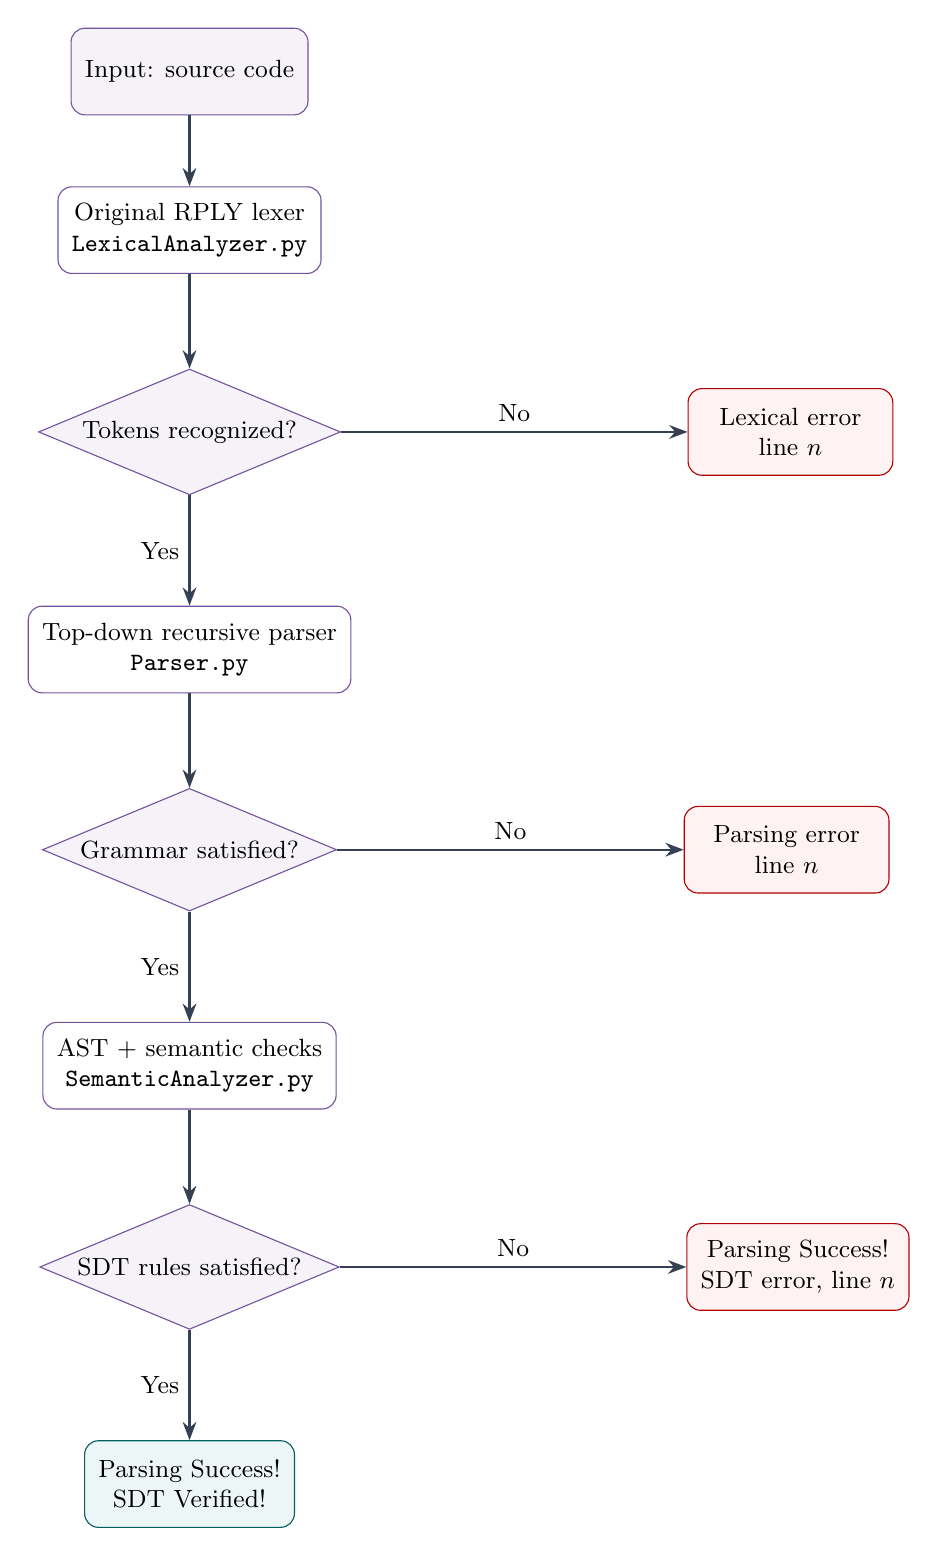
\begin{tikzpicture}[node distance=9mm,font=\small]
\node[state] (input) {Input: source code};
\node[action,below=of input] (lexer) {Original RPLY lexer\\\texttt{LexicalAnalyzer.py}};
\node[decision,below=12mm of lexer] (lexok) {Tokens recognized?};
\node[action,below=14mm of lexok] (parser) {Top-down recursive parser\\\texttt{Parser.py}};
\node[decision,below=12mm of parser] (parseok) {Grammar satisfied?};
\node[action,below=14mm of parseok] (sdt) {AST + semantic checks\\\texttt{SemanticAnalyzer.py}};
\node[decision,below=12mm of sdt] (semok) {SDT rules satisfied?};
\node[success,below=14mm of semok] (ok) {Parsing Success!\\SDT Verified!};
\node[failure,right=44mm of lexok] (le) {Lexical error\\line $n$};
\node[failure,right=44mm of parseok] (pe) {Parsing error\\line $n$};
\node[failure,right=44mm of semok] (se) {Parsing Success!\\SDT error, line $n$};
\draw[arrow] (input)--(lexer);
\draw[arrow] (lexer)--(lexok);
\draw[arrow] (lexok)--node[left]{Yes}(parser);
\draw[arrow] (parser)--(parseok);
\draw[arrow] (parseok)--node[left]{Yes}(sdt);
\draw[arrow] (sdt)--(semok);
\draw[arrow] (semok)--node[left]{Yes}(ok);
\draw[arrow] (lexok)--node[above]{No}(le);
\draw[arrow] (parseok)--node[above]{No}(pe);
\draw[arrow] (semok)--node[above]{No}(se);
\end{tikzpicture}

\end{document}
